\documentclass[12pt]{article}
\usepackage[utf8]{inputenc}
\usepackage{float}
\usepackage{amsmath}
\usepackage{tikz}


\usepackage[hmargin=3cm,vmargin=6.0cm]{geometry}
%\topmargin=0cm
\topmargin=-2cm
\addtolength{\textheight}{6.5cm}
\addtolength{\textwidth}{2.0cm}
%\setlength{\leftmargin}{-5cm}
\setlength{\oddsidemargin}{0.0cm}
\setlength{\evensidemargin}{0.0cm}

%misc libraries goes here



\begin{document}

\section*{Student Information } 
%Write your full name and id number between the colon and newline
%Put one empty space character after colon and before newline
Full Name : Hasan Küreli\\
Id Number :  2580751\\

% Write your answers below the section tags
\section*{Answer 1}
\subsection*{a) }
$$deg(a)=3, deg(b)=3, deg(c)=3, deg(d)=2, deg(e)=3,sum= 14 $$

\subsection*{b) }
Adjacency matrix, Columns and rows are a, b, c, d, e:\\\\
$$\begin{bmatrix}
0 & 1 & 1 & 0 & 1\\
1 & 0 & 1 & 0 & 1\\
1 & 1 & 0 & 1 & 0\\
0 & 0 & 1 & 0 & 1\\
1 & 1 & 0 & 1 & 0 
\end{bmatrix}$$\\
There are 14 non-zero entries.

\subsection*{c) }
Incidence matrix, Columns are edges: \{a,b\}, \{a,c\}, \{a,e\}, \{b,c\}, \{b,e\}, \{c,d\}, \{e,d\\
Rows are vertices: a, b, c, d, e respectively.\\\\
$$\begin{bmatrix}
1 & 1 & 1 & 0 & 0 & 0 & 0\\
1 & 0 & 0 & 1 & 1 & 0 & 0\\
0 & 1 & 0 & 0 & 1 & 1 & 0\\
0 & 0 & 0 & 0 & 0 & 1 & 1\\
0 & 0 & 1 & 1 & 0 & 0 & 1\\
\end{bmatrix}$$\\
There are 21 zero entries.


\subsection*{d) }
No. The adjacency matrix of a complete graph has all non-zero enties except for the diagonal. But if we try to remove any one of the vertices (just 1) and remove corresponding rows and columns in the matrix in part (b) we can't reach this form.

\subsection*{e) }
No. Let's start giving colors blue and red for the vertices with the condition that no adjacent vertex has the same color. Color b red, a blue, c red, we can see it is not bipartite because b and c are adjacent but have the same color red. So, it is not bipartite.

\subsection*{f) }
A directed graph might have each of its edges directed in two different ways. Since, G has 7 edges $2^7=128$ different directed graphs have G as their underlying undirected graph.

\subsection*{g) }
a-b-c-d-e-a-c is the path.\\
The length is 6.

\subsection*{h) }
1. Since G is a connected graph there is only 1 connected component.

\subsection*{i) }
No. Because, G has 4 vertices with odd degree it should have 0.\\

\subsection*{j) }
No. Because, G has 4 vertices with odd degree vertices it should have 0 or 2.

\subsection*{k) }
Yes. The circuit is: a-e-d-c-b-a.

\subsection*{l) }
Yes. The path is: a-e-d-c-b.

\section*{Answer 2}
They are isomorphic.\\
Because we can find a one-to-one and onto function $f$ from G to H such that:\\
$f(a) = a^{'}$\\
$f(b) = b^{'}$\\
$f(c) = c^{'}$\\
$f(d) = d^{'}$\\
$f(e) = e^{'}$\\
And all edges in G are also there in H using this function (a and b are adjacent so is f(a) and f(b)).

\section*{Answer 3}
Visited: A set of the visited vertices which we will not consider again.\\
Unvisited: A set of unvisited vertices.\\
Distance: array that stores distance of each vertex.\\
Previous: array that stores the previous of each vertex.\\


0)
We initialize distance of s to 0 and other to infinity. Add all elements to Unvisited. \\
$\begin{tabular}{|c|c|c|}
\hline
     Vertex & Distance & Previous \\
\hline
    $s$ & 0 & NULL\\
\hline
    $t$ & $\infty$ & NULL\\
\hline
    $u$ & $\infty$ & NULL\\
\hline
    $v$ & $\infty$ & NULL\\
\hline
    $w$ & $\infty$ & NULL\\
\hline
    $x$ & $\infty$ & NULL\\
\hline
    $y$ & $\infty$ & NULL\\
\hline
    $z$ & $\infty$ & NULL\\
\hline
\end{tabular}\\$

Visited = \{\}\\
Unvisited= \{ s,t,u,v,w,x,y,z\}\\

1)
We check the unvisited neigbours of the unvisited vertex with minimum distance which is s and update their distance (if the new distance is lower) and previous. Move s to visited.\\
$\begin{tabular}{|c|c|c|}
\hline
     Vertex & Distance & Previous \\
\hline
    $s$ & 0 & NULL\\
\hline
    $t$ & $\infty$ & NULL\\
\hline
    $u$ & 4 & s\\
\hline
    $v$ & 5 & s\\
\hline
    $w$ & 3 & s\\
\hline
    $x$ & $\infty$ & NULL\\
\hline
    $y$ & $\infty$ & NULL\\
\hline
    $z$ & $\infty$ & NULL\\
\hline
\end{tabular}\\$

Visited = \{s\}\\
Unvisited= \{ t,u,v,w,x,y,z\}\\

2)
We check the neigbours of the unvisited vertex with minimum distance which is w and update their distance and previous. Move w to visited.\\
$\begin{tabular}{|c|c|c|}
\hline
     Vertex & Distance & Previous \\
\hline
    $s$ & 0 & NULL\\
\hline
    $t$ & $\infty$ & NULL\\
\hline
    $u$ & 4 & s\\
\hline
    $v$ & 5 & s\\
\hline
    $w$ & 3 & s\\
\hline
    $x$ & 11 & w\\
\hline
    $y$ & $\infty$ & NULL\\
\hline
    $z$ & 15 & w\\
\hline
\end{tabular}\\$

Visited = \{s,w\}\\
Unvisited= \{ t,u,v,x,y,z\}\\

3)
We check the neigbours of the unvisited vertex with minimum distance which is u and update their distance and previous. Move u to visited.\\
$\begin{tabular}{|c|c|c|}
\hline
     Vertex & Distance & Previous \\
\hline
    $s$ & 0 & NULL\\
\hline
    $t$ & $\infty$ & NULL\\
\hline
    $u$ & 4 & s\\
\hline
    $v$ & 5 & s\\
\hline
    $w$ & 3 & s\\
\hline
    $x$ & 11 & w\\
\hline
    $y$ & 15 & u\\
\hline
    $z$ & 15 & w\\
\hline
\end{tabular}\\$

Visited = \{s,w,u\}\\
Unvisited= \{ t,v,x,y,z\}\\

4)
We check the neigbours of the unvisited vertex with minimum distance which is v and update their distance and previous. Move v to visited.\\
$\begin{tabular}{|c|c|c|}
\hline
     Vertex & Distance & Previous \\
\hline
    $s$ & 0 & NULL\\
\hline
    $t$ & $\infty$ & NULL\\
\hline
    $u$ & 4 & s\\
\hline
    $v$ & 5 & s\\
\hline
    $w$ & 3 & s\\
\hline
    $x$ & 7 & v\\
\hline
    $y$ & 11 & v\\
\hline
    $z$ & 15 & w\\
\hline
\end{tabular}\\$

Visited = \{s,w,u,v\}\\
Unvisited= \{ t,x,y,z\}\\

5)
We check the neigbours of the unvisited vertex with minimum distance which is x and update their distance and previous. Move x to visited.\\
$\begin{tabular}{|c|c|c|}
\hline
     Vertex & Distance & Previous \\
\hline
    $s$ & 0 & NULL\\
\hline
    $t$ & $\infty$ & NULL\\
\hline
    $u$ & 4 & s\\
\hline
    $v$ & 5 & s\\
\hline
    $w$ & 3 & s\\
\hline
    $x$ & 7 & v\\
\hline
    $y$ & 8 & x\\
\hline
    $z$ & 13 & x\\
\hline
\end{tabular}\\$

Visited = \{s,w,u,v,x\}\\
Unvisited= \{ t,y,z\}\\

6)
We check the neigbours of the unvisited vertex with minimum distance which is y and update their distance and previous. Move y to visited.\\
$\begin{tabular}{|c|c|c|}
\hline
     Vertex & Distance & Previous \\
\hline
    $s$ & 0 & NULL\\
\hline
    $t$ & 17 & y\\
\hline
    $u$ & 4 & s\\
\hline
    $v$ & 5 & s\\
\hline
    $w$ & 3 & s\\
\hline
    $x$ & 7 & v\\
\hline
    $y$ & 8 & x\\
\hline
    $z$ & 12 & y\\
\hline
\end{tabular}\\$

Visited = \{s,w,u,v,x,y\}\\
Unvisited= \{ t,z\}\\


7)
We check the neigbours of the unvisited vertex with minimum distance which is z and update their distance and previous. Move z to visited.\\
$\begin{tabular}{|c|c|c|}
\hline
     Vertex & Distance & Previous \\
\hline
    $s$ & 0 & NULL\\
\hline
    $t$ & 15 & z\\
\hline
    $u$ & 4 & s\\
\hline
    $v$ & 5 & s\\
\hline
    $w$ & 3 & s\\
\hline
    $x$ & 7 & v\\
\hline
    $y$ & 8 & x\\
\hline
    $z$ & 12 & y\\
\hline
\end{tabular}\\$

Visited = \{s,w,u,v,x,y,z\}\\
Unvisited= \{ t\}\\
We have reached vertex t so we can stop.\\
The shortest path is found by following the previous:\\
s-v-x-y-z-t\\
distance is 15\\




\section*{Answer 4}
\subsection*{a) }
I will use Kruskal's algorithm.\\
I remove all the edges then start adding them from the edges with minimum weight.\\
There are multiple edges with weight 2. I add them by checking that they don't form any loops.\\
The graph looks like below after this:\\
\begin{figure}[H]
	\centering
	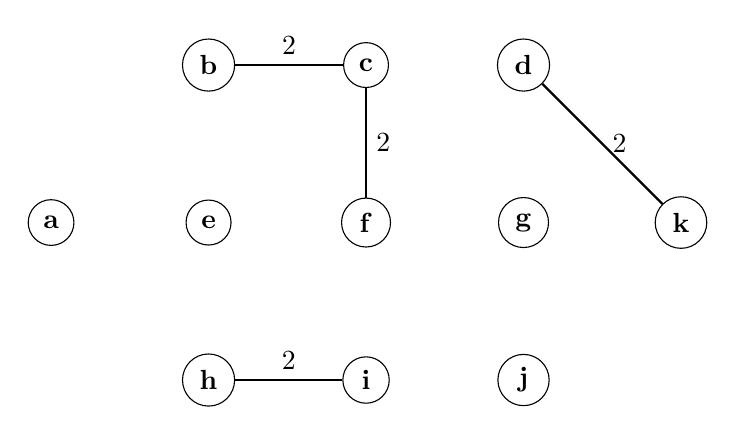
\begin{tikzpicture}
	
	\node[shape=circle,draw=black] (a) at (-2, 2)     {\textbf{a}};
	\node[shape=circle,draw=black] (b) at (0, 4)     {\textbf{b}};
	\node[shape=circle,draw=black] (c) at (2, 4)     {\textbf{c}};
	\node[shape=circle,draw=black] (d) at (4, 4)     {\textbf{d}};
	\node[shape=circle,draw=black] (e) at (0, 2)     {\textbf{e}};
	\node[shape=circle,draw=black] (f) at (2, 2)     {\textbf{f}};
	\node[shape=circle,draw=black] (g) at (4, 2)     {\textbf{g}};
	\node[shape=circle,draw=black] (h) at (0, 0)     {\textbf{h}};
	\node[shape=circle,draw=black] (i) at (2, 0)     {\textbf{i}};
	\node[shape=circle,draw=black] (j) at (4, 0)     {\textbf{j}};
	\node[shape=circle,draw=black] (k) at (6, 2)     {\textbf{k}};
	
	\
	\path[-, thick] (b) edge node[above]{2} (c);
	
	\path[-, thick] (c) edge node[right]{2} (f);
	
	\path[-, thick] (d) edge node[right]{2} (k);
	
	\path[-, thick] (h) edge node[above]{2} (i);
	
	
	\end{tikzpicture} 
	\caption{After some edges are added}	
	\label{fig:g4}
\end{figure}
And then I continue adding the remaining edges with minimum weight by checking the loop condition.\\
The order I add them will be : \{b,c\}, \{c,f\}, \{h,i\}, \{d,k\}, \{c,d\},\{a,b\},\{f,j\}, \{f,i\}, \{e,f\}, and lastly either \{g,j\} or \{f,g\} I choose \{f,g\} \\
Note: The question did not ask to draw all the steps so I did not show all steps clearly. But I just drew an intermediate step.


\subsection*{b) }
\begin{figure}[H]
	\centering
	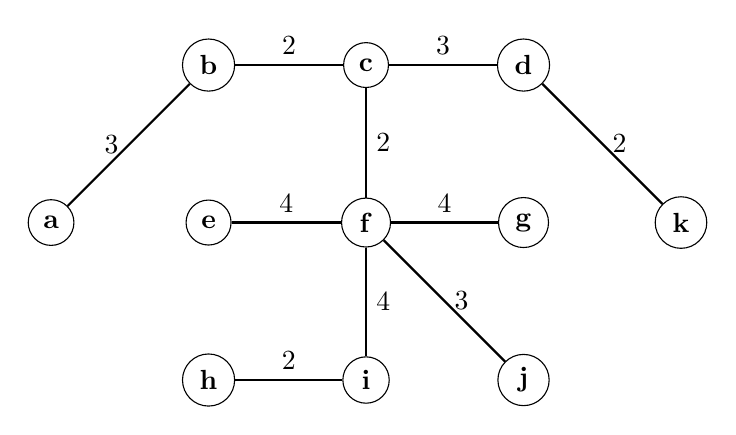
\begin{tikzpicture}
	
	\node[shape=circle,draw=black] (a) at (-2, 2)     {\textbf{a}};
	\node[shape=circle,draw=black] (b) at (0, 4)     {\textbf{b}};
	\node[shape=circle,draw=black] (c) at (2, 4)     {\textbf{c}};
	\node[shape=circle,draw=black] (d) at (4, 4)     {\textbf{d}};
	\node[shape=circle,draw=black] (e) at (0, 2)     {\textbf{e}};
	\node[shape=circle,draw=black] (f) at (2, 2)     {\textbf{f}};
	\node[shape=circle,draw=black] (g) at (4, 2)     {\textbf{g}};
	\node[shape=circle,draw=black] (h) at (0, 0)     {\textbf{h}};
	\node[shape=circle,draw=black] (i) at (2, 0)     {\textbf{i}};
	\node[shape=circle,draw=black] (j) at (4, 0)     {\textbf{j}};
	\node[shape=circle,draw=black] (k) at (6, 2)     {\textbf{k}};
	
	\path[-, thick] (a) edge node[left]{3} (b);
	\path[-, thick] (b) edge node[above]{2} (c);
	\path[-, thick] (c) edge node[above]{3} (d);
	\path[-, thick] (c) edge node[right]{2} (f);
	\path[-, thick] (d) edge node[right]{2} (k);
	\path[-, thick] (e) edge node[above]{4} (f);
	\path[-, thick] (f) edge node[above]{4} (g);
	\path[-, thick] (f) edge node[right]{4} (i);
	\path[-, thick] (f) edge node[right]{3} (j);
	\path[-, thick] (h) edge node[above]{2} (i);
	
	\end{tikzpicture} 
	\caption{The minimum spanning tree}	
	\label{fig:g4}
\end{figure}


\subsection*{c) }
No it is not. I said in part(a) that at the last step I can add two different edges \{g,j\} or \{f,g\} this choice will result in different minimum spanning trees. Hence, it is not unique.

\end{document}